%Version 3.1 December 2024
% See section 11 of the User Manual for version history
%
%%%%%%%%%%%%%%%%%%%%%%%%%%%%%%%%%%%%%%%%%%%%%%%%%%%%%%%%%%%%%%%%%%%%%%
%%                                                                 %%
%% Please do not use \input{...} to include other tex files.       %%
%% Submit your LaTeX manuscript as one .tex document.              %%
%%                                                                 %%
%% All additional figures and files should be attached             %%
%% separately and not embedded in the \TeX\ document itself.       %%
%%                                                                 %%
%%%%%%%%%%%%%%%%%%%%%%%%%%%%%%%%%%%%%%%%%%%%%%%%%%%%%%%%%%%%%%%%%%%%%

%%\documentclass[referee,sn-basic]{sn-jnl}% referee option is meant for double line spacing

%%=======================================================%%
%% to print line numbers in the margin use lineno option %%
%%=======================================================%%

%%\documentclass[lineno,pdflatex,sn-basic]{sn-jnl}% Basic Springer Nature Reference Style/Chemistry Reference Style

%%=========================================================================================%%
%% the documentclass is set to pdflatex as default. You can delete it if not appropriate.  %%
%%=========================================================================================%%

%%\documentclass[sn-basic]{sn-jnl}% Basic Springer Nature Reference Style/Chemistry Reference Style

%%Note: the following reference styles support Namedate and Numbered referencing. By default the style follows the most common style. To switch between the options you can add or remove �Numbered� in the optional parenthesis. 
%%The option is available for: sn-basic.bst, sn-chicago.bst%  
 
%%\documentclass[pdflatex,sn-nature]{sn-jnl}% Style for submissions to Nature Portfolio journals
%%\documentclass[pdflatex,sn-basic]{sn-jnl}% Basic Springer Nature Reference Style/Chemistry Reference Style
\documentclass[pdflatex,sn-mathphys-num]{sn-jnl}% Math and Physical Sciences Numbered Reference Style
%%\documentclass[pdflatex,sn-mathphys-ay]{sn-jnl}% Math and Physical Sciences Author Year Reference Style
%%\documentclass[pdflatex,sn-aps]{sn-jnl}% American Physical Society (APS) Reference Style
%%\documentclass[pdflatex,sn-vancouver-num]{sn-jnl}% Vancouver Numbered Reference Style
%%\documentclass[pdflatex,sn-vancouver-ay]{sn-jnl}% Vancouver Author Year Reference Style
%%\documentclass[pdflatex,sn-apa]{sn-jnl}% APA Reference Style
%%\documentclass[pdflatex,sn-chicago]{sn-jnl}% Chicago-based Humanities Reference Style

%%%% Standard Packages
%%<additional latex packages if required can be included here>

\usepackage{graphicx}%
\usepackage{multirow}%
\usepackage{amsmath,amssymb,amsfonts}%
\usepackage{amsthm}%
\usepackage{mathrsfs}%
\usepackage[title]{appendix}%
\usepackage{xcolor}%
\usepackage{textcomp}%
\usepackage{manyfoot}%
\usepackage{booktabs}%
\usepackage{algorithm}%
\usepackage{algorithmicx}%
\usepackage{algpseudocode}%
\usepackage{listings}%
%%%%

%%%%%=============================================================================%%%%
%%%%  Remarks: This template is provided to aid authors with the preparation
%%%%  of original research articles intended for submission to journals published 
%%%%  by Springer Nature. The guidance has been prepared in partnership with 
%%%%  production teams to conform to Springer Nature technical requirements. 
%%%%  Editorial and presentation requirements differ among journal portfolios and 
%%%%  research disciplines. You may find sections in this template are irrelevant 
%%%%  to your work and are empowered to omit any such section if allowed by the 
%%%%  journal you intend to submit to. The submission guidelines and policies 
%%%%  of the journal take precedence. A detailed User Manual is available in the 
%%%%  template package for technical guidance.
%%%%%=============================================================================%%%%

%% as per the requirement new theorem styles can be included as shown below
\theoremstyle{thmstyleone}%
\newtheorem{theorem}{Theorem}%  meant for continuous numbers
%%\newtheorem{theorem}{Theorem}[section]% meant for sectionwise numbers
%% optional argument [theorem] produces theorem numbering sequence instead of independent numbers for Proposition
\newtheorem{proposition}[theorem]{Proposition}% 
%%\newtheorem{proposition}{Proposition}% to get separate numbers for theorem and proposition etc.

\theoremstyle{thmstyletwo}%
\newtheorem{example}{Example}%
\newtheorem{remark}{Remark}%

\theoremstyle{thmstylethree}%
\newtheorem{definition}{Definition}%

\raggedbottom
%%\unnumbered% uncomment this for unnumbered level heads


\usepackage{xurl}
\newcommand{\NltkVersion}{3.7}
\newcommand{\RealCheckCases}{6}
\newcommand{\IterativeCases}{18}
\newcommand{\IterativeSteps}{1000}
\newcommand{\IterativeSeeds}{3}
\newcommand{\IterativeFreeFraction}{0.50}
\newcommand{\ZipfObservedMin}{450}
\newcommand{\ZipfObservedMax}{467}
\newcommand{\ZipfObservedMean}{459.4}
\newcommand{\IndependentKeywords}{6}
\newcommand{\IndependentDocuments}{200}
\newcommand{\NearDuplicateThreshold}{0.80}
\newcommand{\NearDuplicatePairs}{0}
\newcommand{\SensitivityPartitions}{3}
\newcommand{\SensitivitySeeds}{3}
\newcommand{\ControlledKeywords}{250}
\newcommand{\SensitivityRuns}{222}
\newcommand{\ProductionSplitSeed}{20260901}
\newcommand{\MatchedSelectionSeed}{20260901}
\newcommand{\BalancedSplitSeed}{20260902}
\newcommand{\SensitivityPartitionSeeds}{20261007, 20261008, 20261009}
\newcommand{\SensitivityAttackSeeds}{0, 1, 2}
\newcommand{\SensitivityPositiveDirections}{3}
\newcommand{\SensitivityDirectionCount}{15}
\newcommand{\BalancedSensitivityMin}{-0.0398}
\newcommand{\BalancedSensitivityMax}{0.1255}
\newcommand{\ENControlledStemZipfDifference}{0.0624}
\newcommand{\LUSControlledStemZipfDifference}{-0.0547}
\newcommand{\ShuffledWeightedMin}{0.0164}
\newcommand{\ShuffledWeightedMax}{0.0802}
\newcommand{\ProductionPairs}{4974}
\newcommand{\Keywords}{500}
\newcommand{\SeedCount}{10}
\newcommand{\ProductionRuns}{120}
\newcommand{\LanguageSignificant}{5}
\newcommand{\PreprocessingSignificant}{11}
\newcommand{\BalancedPairs}{253}
\newcommand{\BalancedSignificant}{6}
\newcommand{\MatchedPairs}{562}
\newcommand{\SourceRows}{50000}
\newcommand{\SentencesPerBlock}{10}
\newcommand{\EnglishStemMatched}{37}
\newcommand{\EnglishStemTotal}{40}
\newcommand{\MizoStemMatched}{41}
\newcommand{\MizoStemTotal}{50}
\newcommand{\UnderStemming}{4}
\newcommand{\OverStemming}{5}
\newcommand{\EnglishStopwords}{116}
\newcommand{\MizoStopwords}{117}
\newcommand{\MizoRules}{15}
\newcommand{\MinimumLetters}{2}
\newcommand{\FinalIterations}{1000}
\newcommand{\QueriesPerKeyword}{10}
\newcommand{\LanguageFamily}{12}
\newcommand{\PreprocessingFamily}{24}
\newcommand{\ConfidencePercent}{95}
\newcommand{\Alpha}{0.05}
\newcommand{\LengthRatio}{1.25}
\newcommand{\FreeFraction}{0.25}
\newcommand{\EnronClient}{20000}
\newcommand{\EnronAuxiliary}{10000}
\newcommand{\InterventionKeywords}{250}
\newcommand{\SimilarityPairs}{31}
\newcommand{\CollisionPairs}{62}
\newcommand{\CandidateBudget}{1}
\newcommand{\EnronMean}{0.9712}
\newcommand{\EnronLow}{0.9611}
\newcommand{\EnronHigh}{0.9813}
\newcommand{\SmokeObserved}{0.972}
\newcommand{\SmokeExpected}{0.952}
\newcommand{\PythonVersion}{3.9.12}
\newcommand{\NumpyVersion}{1.22.3}
\newcommand{\ScipyVersion}{1.8.0}
\newcommand{\UpstreamRevision}{10631a10e3ec461ad01d38fc74f7933d31062ba5}
\newcommand{\IdenticalPairs}{0}
\newcommand{\ENTokenUniformPercent}{13.45}
\newcommand{\ENStopUniformPercent}{5.75}
\newcommand{\ENStemUniformPercent}{5.35}
\newcommand{\ENTokenZipfWeighted}{0.5907}
\newcommand{\ENTokenZipfMacro}{0.1485}
\newcommand{\LUSTokenUniformPercent}{11.91}
\newcommand{\LUSStopUniformPercent}{6.95}
\newcommand{\LUSStemUniformPercent}{7.19}
\newcommand{\LUSTokenZipfWeighted}{0.5617}
\newcommand{\LUSTokenZipfMacro}{0.1129}
\newcommand{\MatchedEnglishDifference}{0.1893}
\newcommand{\MatchedEnglishP}{0.0156}
\newcommand{\WMTMarkerEN}{67.59}
\newcommand{\WMTMarkerLUS}{78.26}
\newcommand{\FloresMarkerEN}{1.19}
\newcommand{\FloresMarkerLUS}{1.98}
\newcommand{\CommitID}{\texttt{1063\allowbreak{}1a10\allowbreak{}e3ec\allowbreak{}461a\allowbreak{}d01d\allowbreak{}38fc\allowbreak{}74f7\allowbreak{}933d\allowbreak{}3106\allowbreak{}2ba5}}
\begin{document}
\title[English-Mizo IHOP Query Recovery]{Corpus and Preprocessing Effects on IHOP Query Recovery in English and Mizo}

\author[1]{\sur{Vanlalhruaia}}\email{mzut160@mzu.edu.in}

\author[2]{\sur{C Lalrinawma}}\email{rinchawngthu777@gmail.com}

\author*[1]{\sur{C Vanlalnunpuia}}\email{mzu230006869@mzu.edu.in}

\author[3]{\sur{Phibansabeth Nongkseh}}\email{phibansabeth@nehu.ac.in}

\author[1]{\sur{R Lalduhsaka}}\email{duskeralte777@gmail.com}

\author[1]{\sur{Zaitinkhuma Thihlum}}\email{zaiamay94@gmail.com}

\affil[1]{\orgdiv{Department of Computer Engineering}, \orgname{Mizoram University}, \orgaddress{\city{Aizawl}, \postcode{796004}}}

\affil[2]{\orgdiv{Department of Information Technology}, \orgname{Mizoram University}, \orgaddress{\city{Aizawl}, \postcode{796004}}}

\affil[3]{\orgdiv{Department of Information Technology}, \orgname{North Eastern Hill University}, \orgaddress{\city{Shillong}, \postcode{793022}}}

\abstract{Query recovery from searchable symmetric encryption was evaluated under matched English-Mizo preprocessing and fixed auxiliary-client partitions. Improved Statistical Query Recovery against Searchable Symmetric Encryption through Quadratic Optimization (IHOP) was applied to \ProductionPairs{} paired text blocks under tokenisation, reviewed stopword removal, and stopword removal with stemming. Each original condition used \Keywords{} selected keywords and \SeedCount{} random seeds. Under uniform queries, mean query-weighted recovery fell from \ENTokenUniformPercent{}\% to \ENStemUniformPercent{}\% in English and from \LUSTokenUniformPercent{}\% to \LUSStemUniformPercent{}\% in Mizo between tokenisation and stemming. \LanguageSignificant{} language comparisons remained statistically significant after Holm correction within the original partition. Additional partitions changed the language-contrast directions. A linked length-balanced control retained \BalancedPairs{} pairs from each corpus. Its English Zipf recovery contrasts also changed sign across additional partitions. Enron matrix interventions produced different recovery effects, with the largest tested reduction under incidence thinning. Preprocessing changed the keyword set as well as its incidence structure. The findings were conditional on partition membership, keyword selection, and the evaluated attack.}

\keywords{searchable symmetric encryption, query recovery, Mizo, preprocessing, corpus evaluation}

\maketitle

\section{Introduction}
Searchable symmetric encryption (SSE) supports keyword retrieval over encrypted document collections~\cite{curtmola}. Search patterns expose repeated queries. Access patterns expose the matching document identifiers. Query-recovery attacks associate these observations with plaintext keywords using auxiliary information~\cite{islam,blackstone}.

Attack evaluations depend on the query space and the information supplied to the adversary. Blackstone et al. examined the assumptions of leakage-abuse attacks across query selectivities, known-data rates, and collections~\cite{blackstone}. The LEAKER framework evaluated attacks on several collections and documented changes in performance under real-world data~\cite{leaker}. These studies motivate explicit reporting of corpus construction and candidate-keyword selection.

Published attacks used different leakage and auxiliary-knowledge assumptions. Cash et al. evaluated leakage-abuse attacks under several levels of server knowledge~\cite{cash}. Damie et al. used non-indexed auxiliary documents and a small set of known queries in a refined score attack~\cite{damie}. Oya and Kerschbaum combined search-pattern and access-pattern observations with query-distribution information in a likelihood-based attack~\cite{sap}. Hoover et al. evaluated leakage-abuse attacks on structured encryption for structured query language (SQL) operations~\cite{hoover}.

IHOP formulates statistical query recovery as a quadratic optimisation problem and iterates over linear assignment solutions~\cite{ihop}. Its volume configuration uses individual response sizes and document co-occurrence. The recovered query labels therefore depend on the indexed document-keyword incidence matrix. Preprocessing changes that matrix when tokens are removed or reduced to stems.

The present evaluation compared English and Mizo representations of aligned text under a shared tokeniser and reviewed language-specific resources. Fixed document pairs and partition membership were retained across preprocessing conditions. A second aligned corpus supplied a corpus-choice sensitivity analysis. Enron matrix interventions supplied separate controlled comparisons of structural changes. The contribution was a conditional evaluation of IHOP across these representations. Generalisation to other attacks and deployment settings was outside the evaluated scope.

\section{Results}
The Enron baseline achieved mean final recovery of \EnronMean{} with a \ConfidencePercent{}\% confidence interval (CI) of [\EnronLow{}, \EnronHigh{}]. The baseline used one query per keyword. The recorded single-seed result was \SmokeObserved{} at the final checkpoint. The upstream reference comment reported \SmokeExpected{}~\cite{ihopcode}. Fixing Python hash ordering left the discrepancy unchanged. The upstream repository documented code cleaning without rerunning every experiment. The cause of the reference mismatch remained unresolved. An independent binomial-likelihood calculation and exhaustive assignment check passed on a planted fixture with \IndependentKeywords{} keywords and \IndependentDocuments{} documents. Assignment costs and exhaustive minima also agreed on \RealCheckCases{} real-data subsets spanning both languages and all preprocessing conditions. Every recorded update was audited in \IterativeCases{} small-fixture runs through \IterativeSteps{} iterations. Production-scale independent equivalence remained unvalidated. The production experiment matched a separate replay exactly. Replay established execution repeatability within the pinned implementation.

Table~\ref{tab:recovery} shows production recovery means and sample standard deviations (SD). Under uniform queries, tokenisation-only query-weighted recovery was \ENTokenUniformPercent{}\% in English and \LUSTokenUniformPercent{}\% in Mizo. Stopword removal reduced these means to \ENStopUniformPercent{}\% and \LUSStopUniformPercent{}\%. The stemming-condition means were \ENStemUniformPercent{}\% and \LUSStemUniformPercent{}\%. Figure~\ref{fig:recovery} shows the checkpoint means.

\begin{table}[htbp]
\centering\small
\caption{Final recovery means and sample standard deviations.}\label{tab:recovery}
\begin{tabular}{@{}lllll@{}}
\toprule
Language & Condition & Queries & Weighted (SD) & Macro (SD) \\
\midrule
English & Tokenisation & Uniform & 0.1345 (0.0192) & 0.1340 (0.0158) \\
English & Tokenisation & Zipf & 0.5907 (0.0667) & 0.1485 (0.0153) \\
English & Stopwords & Uniform & 0.0575 (0.0096) & 0.0570 (0.0103) \\
English & Stopwords & Zipf & 0.4695 (0.0276) & 0.0655 (0.0112) \\
English & Stemming & Uniform & 0.0535 (0.0069) & 0.0528 (0.0071) \\
English & Stemming & Zipf & 0.3960 (0.0714) & 0.0572 (0.0070) \\
Mizo & Tokenisation & Uniform & 0.1191 (0.0204) & 0.1196 (0.0176) \\
Mizo & Tokenisation & Zipf & 0.5617 (0.0304) & 0.1129 (0.0276) \\
Mizo & Stopwords & Uniform & 0.0695 (0.0089) & 0.0698 (0.0071) \\
Mizo & Stopwords & Zipf & 0.5468 (0.0435) & 0.0788 (0.0132) \\
Mizo & Stemming & Uniform & 0.0719 (0.0134) & 0.0728 (0.0116) \\
Mizo & Stemming & Zipf & 0.5340 (0.0261) & 0.0783 (0.0111) \\
\botrule
\end{tabular}
\end{table}

\begin{figure}[htbp]
\centering
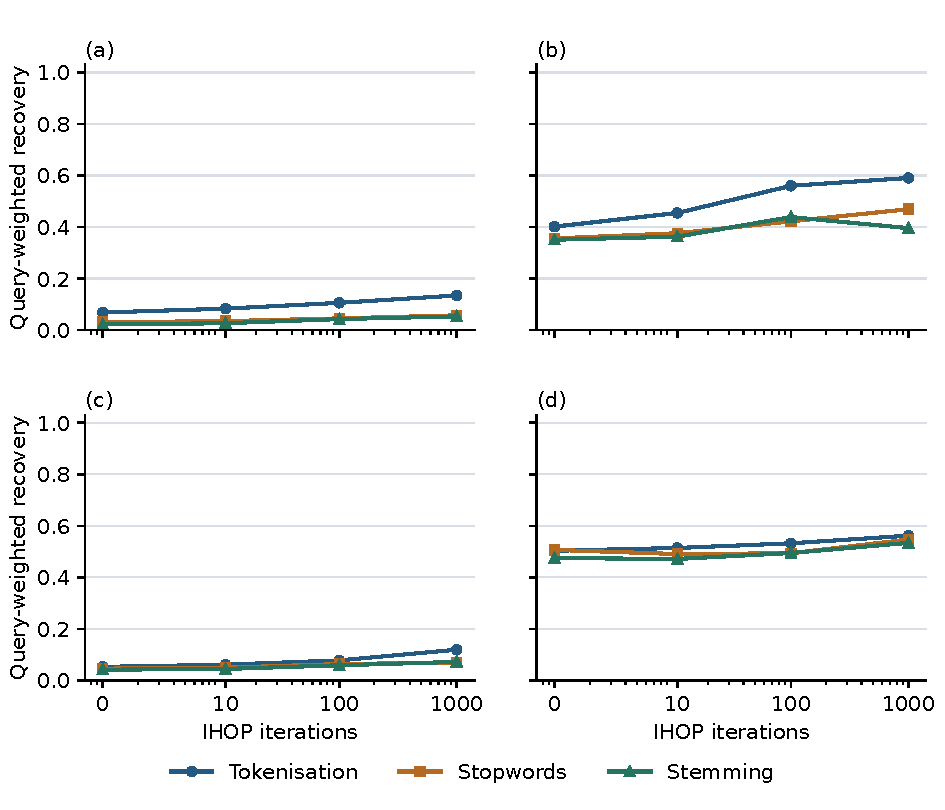
\includegraphics[width=\textwidth]{Fig1.pdf}
\caption{Mean query-weighted recovery by iteration. (a) English uniform. (b) English Zipf. (c) Mizo uniform. (d) Mizo Zipf. Symbols identify preprocessing}
\label{fig:recovery}
\end{figure}

Zipf queries produced different weighted and macro recovery measurements. English tokenisation-only query-weighted recovery was \ENTokenZipfWeighted{}, and keyword-macro recovery was \ENTokenZipfMacro{}. The corresponding Mizo measurements were \LUSTokenZipfWeighted{} and \LUSTokenZipfMacro{} (Table~\ref{tab:recovery}). The weighted measurement assigned more observations to higher-ranked keywords. The macro measurement assigned equal weight to each observed distinct keyword.

Uniform runs observed all \Keywords{} keywords. Zipf runs observed \ZipfObservedMin{}-\ZipfObservedMax{} keywords, with a mean of \ZipfObservedMean{} (Supplementary Table S10). Query generation therefore changed the observed assignment problem and the scoring weights. The macro denominator contained only observed keywords.

Table~\ref{tab:language} reports paired language differences. \LanguageSignificant{} comparisons had Holm-adjusted probabilities below \Alpha{}. Mizo recovery was higher for Zipf query-weighted recovery after stopword removal. After stemming, Mizo recovery was higher for both recovery measurements under both query distributions. The tokenisation-only language comparisons remained above the corrected threshold. The additional preprocessing contrasts were supplied in the supplementary tables. \PreprocessingSignificant{} contrasts remained below the corrected threshold. The stemmed versus stopword-only contrasts remained above it.

\begin{table}[htbp]
\centering\small
\caption{Mizo minus English recovery at the final checkpoint.}\label{tab:language}
\begin{tabular}{@{}lllrrr@{}}
\toprule
Condition & Queries & Metric & Difference & 95\% CI$^{a}$ & Holm $p$ \\
\midrule
Tokenisation & Uniform & Weighted & -0.0155 & \shortstack{[-0.0305,\\-0.0004]} & 0.1406 \\
Tokenisation & Uniform & Macro & -0.0144 & \shortstack{[-0.0260,\\-0.0028]} & 0.0820 \\
Tokenisation & Zipf & Weighted & -0.0290 & \shortstack{[-0.0731,\\0.0152]} & 0.1621 \\
Tokenisation & Zipf & Macro & -0.0356 & \shortstack{[-0.0604,\\-0.0107]} & 0.0820 \\
Stopwords & Uniform & Weighted & 0.0120 & \shortstack{[0.0029,\\0.0212]} & 0.0820 \\
Stopwords & Uniform & Macro & 0.0128 & \shortstack{[0.0034,\\0.0222]} & 0.0820 \\
Stopwords & Zipf & Weighted & 0.0773 & \shortstack{[0.0392,\\0.1154]} & 0.0234 \\
Stopwords & Zipf & Macro & 0.0133 & \shortstack{[0.0006,\\0.0259]} & 0.1406 \\
Stemming & Uniform & Weighted & 0.0184 & \shortstack{[0.0072,\\0.0297]} & 0.0312 \\
Stemming & Uniform & Macro & 0.0200 & \shortstack{[0.0102,\\0.0298]} & 0.0234 \\
Stemming & Zipf & Weighted & 0.1380 & \shortstack{[0.0955,\\0.1805]} & 0.0234 \\
Stemming & Zipf & Macro & 0.0211 & \shortstack{[0.0129,\\0.0294]} & 0.0234 \\
\botrule
\end{tabular}\par\footnotesize $^{a}$Unadjusted confidence intervals.
\end{table}

Post-review sensitivity analyses used \SensitivityPartitions{} additional paired partitions and \SensitivitySeeds{} attack seeds per condition. The original statistically significant language comparisons had positive Mizo-minus-English partition means in \SensitivityPositiveDirections{} of \SensitivityDirectionCount{} additional comparisons. Figure~\ref{fig:partition} shows contrasts using matched attack seeds in the original and additional partitions. Supplementary Tables S11, S14, and S15 report seed variation and paired contrasts. These comparisons were descriptive.

\begin{figure}[htbp]
\centering
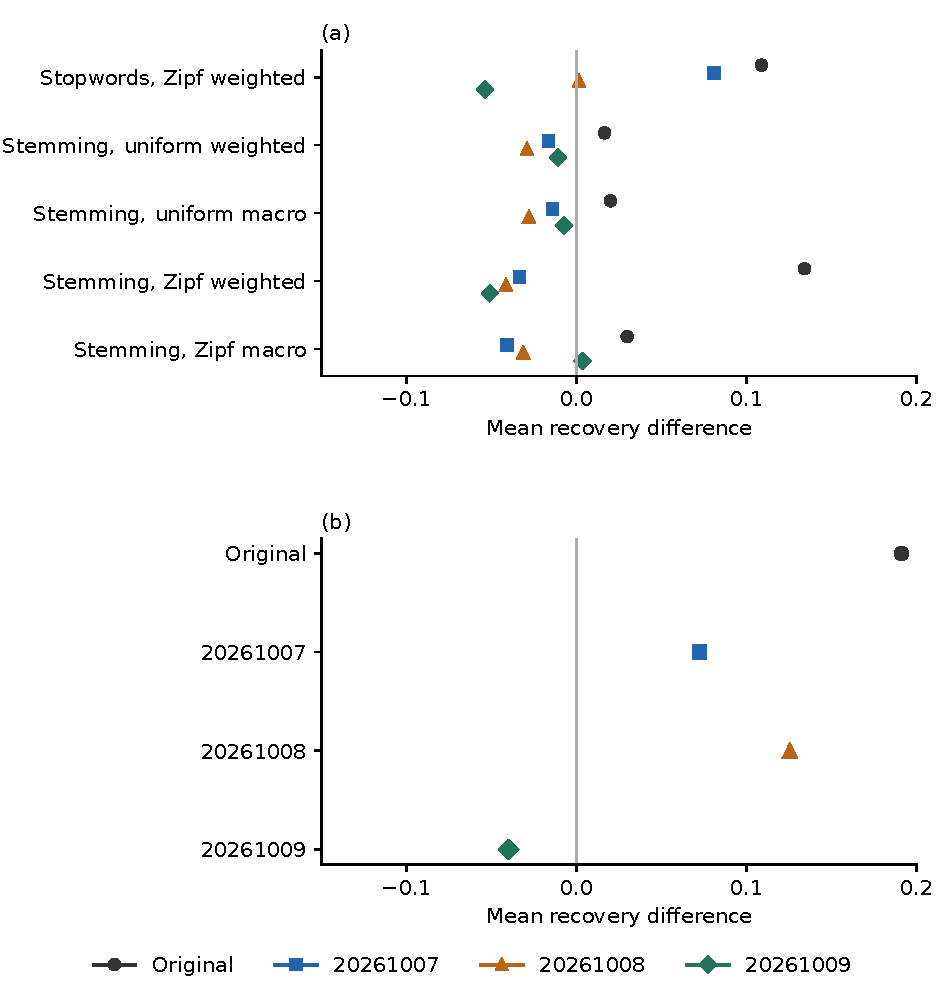
\includegraphics[width=\textwidth]{Fig2.pdf}
\caption{Selected partition mean contrasts. (a) Mizo minus English. (b) English length-balanced Zipf query-weighted FLORES minus WMT23. Symbols identify partitions}
\label{fig:partition}
\end{figure}

Table~\ref{tab:structure} shows structure in the exact production client indexes. The identical-access-pair count was \IdenticalPairs{} across all production keyword sets. Stopword removal increased the proportion of keywords with an equal-frequency alternative in both languages. Mean recovery also fell under uniform queries (Table~\ref{tab:recovery}). Density and the selected vocabulary changed concurrently. These observations did not isolate frequency ambiguity as the sole mechanism.

\begin{table}[htbp]
\centering\small
\caption{Client-index density, frequency alternatives, and median similarities.}\label{tab:structure}
\begin{tabular}{@{}llrrrr@{}}
\toprule
Language & Condition & Density & Alternatives & Nearest Jaccard & Cosine \\
\midrule
English & Tokenisation & 0.1376 & 0.5800 & 0.1057 & 0.9883 \\
English & Stopwords & 0.0663 & 0.7440 & 0.0804 & 0.9451 \\
English & Stemming & 0.0766 & 0.7300 & 0.0870 & 0.9583 \\
Mizo & Tokenisation & 0.1435 & 0.5420 & 0.1184 & 0.9890 \\
Mizo & Stopwords & 0.0793 & 0.7220 & 0.0858 & 0.9668 \\
Mizo & Stemming & 0.0901 & 0.6660 & 0.0958 & 0.9722 \\
\botrule
\end{tabular}
\end{table}

The matched-size corpus comparison used \MatchedPairs{} pairs per collection. English Zipf query-weighted recovery was \MatchedEnglishDifference{} higher in FLORES-200, with Holm-adjusted probability \MatchedEnglishP{}. After bilingual length balancing, \BalancedPairs{} cross-corpus pairs remained. Table~\ref{tab:balanced} shows selected Zipf query-weighted contrasts. The English differences remained positive and below the corrected threshold across the evaluated keyword sizes. \BalancedSignificant{} of the full comparison set remained below that threshold. All of those comparisons concerned English. The full set included both query distributions and both recovery measurements.

\begin{table}[htbp]
\centering\small
\caption{Selected Zipf query-weighted recovery contrasts after length balancing.}\label{tab:balanced}
\begin{tabular}{@{}lrrrrrr@{}}
\toprule
Language & $K$ & FLORES & WMT23 & Difference & 95\% CI$^{a}$ & Holm $p$ \\
\midrule
English & 100 & 0.3983 & 0.1196 & 0.2787 & \shortstack{[0.2038,\\0.3536]} & 0.0469 \\
Mizo & 100 & 0.4313 & 0.3483 & 0.0830 & \shortstack{[-0.0215,\\0.1875]} & 0.3398 \\
English & 250 & 0.3658 & 0.1103 & 0.2555 & \shortstack{[0.2128,\\0.2983]} & 0.0469 \\
Mizo & 250 & 0.3560 & 0.2652 & 0.0908 & \shortstack{[-0.0122,\\0.1938]} & 0.3398 \\
English & 500 & 0.2955 & 0.1246 & 0.1709 & \shortstack{[0.1187,\\0.2231]} & 0.0469 \\
Mizo & 500 & 0.2813 & 0.1793 & 0.1020 & \shortstack{[0.0119,\\0.1920]} & 0.2734 \\
\botrule
\end{tabular}\par\footnotesize $^{a}$Unadjusted confidence intervals.
\end{table}

English length-balanced Zipf query-weighted FLORES-minus-WMT23 differences ranged from \BalancedSensitivityMin{} to \BalancedSensitivityMax{} at \Keywords{} keywords across additional partitions (Figure~\ref{fig:partition}). Supplementary Tables S13 and S14 report recovery means and paired contrasts with sample standard deviations. The corpus ordering changed across the configured partitions.

Religious-marker screening identified different lexical compositions in the length-balanced collections. Marker prevalence was \WMTMarkerEN{}\% in WMT23 English and \WMTMarkerLUS{}\% in WMT23 Mizo. The corresponding FLORES-200 percentages were \FloresMarkerEN{}\% and \FloresMarkerLUS{}\%. Screening measured the occurrence of specified tokens. It did not classify every document's domain. Corpus construction and source composition remained different after length balancing.

Table~\ref{tab:ablation} shows paired Enron intervention endpoints. Incidence thinning had the largest negative mean endpoint contrast. Frequency equality and exact access collisions also reduced recovery. Frequency-preserving access similarity produced a smaller negative contrast. The keyword-count and co-occurrence endpoints had intervals that included zero. Intervention scales differed across rows. The endpoint values therefore described each configured intervention separately.

\begin{sidewaystable}[htbp]
\centering\small
\caption{Paired final-recovery differences at the configured Enron intervention endpoints.}\label{tab:ablation}
\begin{tabular}{@{}p{29mm}p{53mm}rr@{}}
\toprule
Intervention & Endpoint contrast & Difference & 95\% CI \\
\midrule
Keyword count & 500 minus 100 keywords & 0.0222 & [-0.0099, 0.0543] \\
Exact access collisions & 62 pairs minus control & -0.2984 & [-0.3914, -0.2054] \\
Access similarity & Jaccard 0.75 minus control & -0.0348 & [-0.0502, -0.0194] \\
Frequency equality & 62 pairs minus control & -0.4816 & [-0.5059, -0.4573] \\
Co-occurrence similarity & Budget 128 minus budget 1 & -0.0008 & [-0.0134, 0.0118] \\
Incidence retention & 25\% minus 100\% retention & -0.8392 & [-0.8620, -0.8164] \\
\botrule
\end{tabular}
\end{sidewaystable}

A controlled candidate set retained \ControlledKeywords{} word labels per language with distinct mapped stems (Supplementary Table S12). Tokenisation-only and stopword-only incidence matrices were identical on these retained terms. The stemming comparison incorporated incidences of all forms mapped to each selected stem. Controlled Zipf query-weighted stemming-minus-stopword differences were \ENControlledStemZipfDifference{} in English and \LUSControlledStemZipfDifference{} in Mizo. Shuffled Zipf ranks were compared with frequency-ranked queries using the same attack seeds (Supplementary Table S12). Shuffled-rank weighted means ranged from \ShuffledWeightedMin{} to \ShuffledWeightedMax{}. These \SensitivityRuns{} runs were descriptive sensitivity analyses.

Cross-partition unigram-set screening found \NearDuplicatePairs{} document pairs at Jaccard similarity of at least \NearDuplicateThreshold{} across the original production partitions. This screen measured lexical overlap. Source-level independence remained unverified because original article identifiers were unavailable.

\section{Methods}
\subsection{Corpora}
The WMT23 IndicNE-Corp archive supplied aligned English-Mizo sentence files~\cite{indic}. The selected training files contained \SourceRows{} aligned rows. Empty text, empty token sequences, and repeated bilingual pairs were excluded. The retained rows were grouped into consecutive blocks of \SentencesPerBlock{} sentence pairs. The final incomplete block was excluded. This produced \ProductionPairs{} paired blocks. Grouping supplied evaluation document boundaries. It did not preserve source article boundaries.

FLORES-200 development and development-test sentences were grouped by source URL~\cite{flores}. The grouping produced \MatchedPairs{} paired excerpts from Wikinews, Wikivoyage, and Wikibooks. The source dataset was distributed under Creative Commons Attribution-ShareAlike 4.0~\cite{floresrepo}. The WMT23 source text remained outside the proposed redistribution package. Acquisition identifiers, source hashes, and construction rules were recorded locally.

Table~\ref{tab:corpora} shows the fixed bilingual partitions. English and Mizo members of each aligned pair were assigned together. Production pairs were ranked by SHA-256 of the partition seed and paired record identifiers. The first auxiliary-sized prefix was assigned to the auxiliary partition. The production partition seed was \ProductionSplitSeed{}. A matched-size WMT23 subset used the FLORES-200 pair count. Pairs were selected by deterministic hash ranking with seed \MatchedSelectionSeed{}.

The length-balanced control used one-to-one assignment without replacement. Eligibility required a maximum token-length ratio of \LengthRatio{} in both languages. Maximum matching cardinality was prioritised. The summed absolute bilingual log-length difference was minimised among eligible assignments. Linked match identifiers were hash-ranked for partition assignment with seed \BalancedSplitSeed{}. Corresponding cross-corpus pairs were assigned to the same partition. All corpus-choice controls used tokenisation only. Original configurations and exact partition indices were included with the derived results.

\begin{table}[htbp]
\centering\small
\caption{Paired collection sizes and fixed partition sizes per language.}\label{tab:corpora}
\begin{tabular}{@{}lrrr@{}}
\toprule
Collection & Pairs & Auxiliary & Client \\
\midrule
WMT23 production & 4974 & 1658 & 3316 \\
FLORES and WMT23 matched & 562 & 187 & 375 \\
FLORES and WMT23 length-balanced & 253 & 84 & 169 \\
\botrule
\end{tabular}
\end{table}

Religious markers were screened in tokenised text. The English marker set contained god, israel, jesus, and lord. The Mizo set contained israel, lalpa, and pathian. A document was counted when at least one marker occurred. This screen described lexical composition in the retained collections. It supplied a reproducible marker count without exhaustive topic annotation.

\subsection{Preprocessing}
Text was normalised to Unicode Normalization Form C (NFC) and case-folded. The tokeniser retained letters, combining marks, and digits. Apostrophes were retained inside letter sequences. Hyphens separated tokens. Numeric-only tokens and tokens with fewer than \MinimumLetters{} letters were excluded. The same tokeniser was applied to both languages.

The preprocessing conditions were tokenisation only, reviewed stopword removal, and reviewed stopword removal followed by stemming. The review accepted \EnglishStopwords{} English and \MizoStopwords{} Mizo stopwords for exclusion. English stemming used the Snowball English (Porter2) algorithm through the Natural Language Toolkit (NLTK) version \NltkVersion{}~\cite{snowball}. The constructor was \texttt{SnowballStemmer("english")}. Mizo stemming used \MizoRules{} reviewed suffix rules. C Lalrinawma, a coauthor, native Mizo speaker, and doctoral researcher in natural language processing, completed the linguistic review. The review supplied token decisions and expected stems. The reviewer subsequently clarified the execution procedure. The reviewed suffix inventory, exceptions, and expected stems were preserved. Supplementary Tables S7 and S8 supplied the complete execution rules and excluded stopword lists.

The annotation sample was purposively selected from frequent, middle-frequency, and infrequent corpus forms. Additional Mizo items covered candidate suffix endings. The sample was used during rule review and execution clarification. Stemming agreement was measured on the reviewed development sample. The original labels were preserved (Supplementary Table S5).

Mizo rules were tried in priority order. Longer suffixes were tried first within a priority. The first eligible rule was applied to the current form. Exceptions blocked only their associated rule, and lower-priority rules remained eligible on that form. Passes were repeated until no rule applied. Every rule shortened the token. Minimum stem length counted written letters with their diacritics. Combining marks did not add letters. Corpus occurrence was excluded from rule eligibility. The annotation disagreements were retained in the supplementary material.

The highest document-frequency eligible keywords were selected separately for each language and preprocessing condition. Lexical order resolved frequency ties. Eligibility required occurrence in a strict subset of both the auxiliary and client partitions. Production experiments used \Keywords{} keywords. Corpus-choice controls additionally used the keyword sizes shown in Table~\ref{tab:balanced}. Selection used the full collection's document frequencies. Both partitions contributed to this evaluation-universe construction.

Each selected document-keyword matrix was binary. Matrix density was the proportion of non-zero entries. Frequency alternatives were keywords whose document frequencies matched those of at least one other selected keyword. Access similarity was Jaccard similarity between binary incidence columns. Co-occurrence profiles were rows of the keyword co-occurrence matrix with their diagonal entries removed. Cosine similarity was measured over distinct profile pairs. Auxiliary-client differences were measured on aligned candidate-keyword probabilities. These statistics were computed from the exact attack exports.

\subsection{Evaluation}
The adversary was a passive server observing unmodified single-keyword access patterns and response volumes. Plaintext auxiliary documents were disjoint from client documents. The candidate-keyword universe was given to the attack. Known query labels were not supplied. Static document collections were used. Dynamic updates and leakage-hiding defences were outside the tested configuration.

The upstream IHOP implementation was pinned to commit \CommitID{}~\cite{ihopcode}. The canonical environment used Python \PythonVersion{}, NumPy \NumpyVersion{}, and SciPy \ScipyVersion{}. The attack used volume mode with free fraction \FreeFraction{}. Production and corpus-choice recovery was evaluated at the configured checkpoints through \FinalIterations{} iterations. Figure~\ref{fig:recovery} used $\log_{10}(i+1)$ iteration spacing.

Each production condition used \SeedCount{} seeds. Uniform and Zipf queries were independent and identically distributed (IID). Uniform probabilities were equal over the selected keyword universe. Zipf probabilities were proportional to inverse rank. Ranks followed the selected document-frequency ordering. Each run generated \QueriesPerKeyword{} times the selected keyword count in query observations. The same seed specifications were used across paired conditions. Auxiliary query probabilities were uniform placeholders. Volume-mode assignment costs excluded query-frequency terms. The free-token count was the integer part of \FreeFraction{} times the observed token count~\cite{ihopcode}. Enron interventions used the recorded one-query-per-keyword configuration. Their recovery scale therefore differed from the generated-query corpus comparisons.

Post-review partition seeds were \SensitivityPartitionSeeds{}. Attack seeds were \SensitivityAttackSeeds{}. Control settings were frozen in a separate configuration before those recovery runs. Bilingual membership remained linked. Length-balanced cross-corpus membership remained linked by match identifier. The original partition means in Figure~\ref{fig:partition} used those same attack seeds. Panel (a) selected the language comparisons significant in the original confirmatory family. Panel (b) used English Zipf query-weighted recovery at \Keywords{} keywords. Controlled word labels were selected in descending stopword-filtered document frequency. Eligibility required support in both partitions and a unique output stem among selected labels. Stemming used the corresponding complete-corpus stem column. A fixed seeded permutation assigned Zipf ranks in the shuffled-rank control. Candidate columns were reordered by that permutation. Original confirmatory results and comparison families were preserved. Supplementary Tables S9-S15 supplied diagnostics and descriptive sensitivity summaries.

The Enron Email Dataset supplied the English email collection~\cite{enrondata}. Its processed representation was supplied by the pinned IHOP repository~\cite{ihopcode}. The Enron experiments used \EnronClient{} client documents and \EnronAuxiliary{} auxiliary documents per seed. Keyword-size experiments used nested prefixes of the same random keyword ordering. Matrix interventions used \InterventionKeywords{} selected keywords. The document partitions, keyword labels, and query order were retained within each paired intervention. Interventions were applied to both client and auxiliary matrices.

Exact access collisions were introduced by assigning identical incidence columns to consecutive selected keyword pairs. The endpoint forced \CollisionPairs{} pairs. Frequency equality was introduced in nearest-frequency pairs with even combined counts. Each pair received its integer mean frequency. Its reconstructed columns had disjoint access sets. Pair totals and overall matrix density were preserved in the frequency-equality intervention.

Access-similarity interventions used \SimilarityPairs{} nearest-frequency pairs feasible in both matrices. Each column's frequency was preserved while pair overlap was changed to the configured Jaccard target. Co-occurrence interventions used the same frequency-preserving pair reconstruction with disjoint pair access sets. Candidate reconstructions were scored by cosine similarity to the donor co-occurrence profile. The highest-scoring candidate was selected. The paired reference used a candidate budget of \CandidateBudget{} and supplied a random reconstruction.

Incidence thinning retained nested deterministic prefixes of each column's incidences. Every column retained at least one incidence. Keyword-frequency weak ordering was preserved. The intervention endpoints and corresponding paired reference settings are listed in Table~\ref{tab:ablation}. Full configurations were retained with the derived results.

For query labels $q_t$ and predictions $\hat q_t$, query-weighted recovery was
\[
R_{\mathrm{weighted}}=\frac{1}{T}\sum_{t=1}^{T}\mathbf{1}(\hat q_t=q_t).
\]
For the observed distinct keyword set $U$, keyword-macro recovery was
\[
R_{\mathrm{macro}}=\frac{1}{|U|}\sum_{u\in U}
\frac{\sum_{t:q_t=u}\mathbf{1}(\hat q_t=u)}{|\{t:q_t=u\}|}.
\]
Unobserved keywords were excluded from the macro denominator. Enron recovery measurements coincided when every keyword was queried once.

Means and sample standard deviations were computed across seeds. Recovery intervals used Student t intervals. Paired contrasts used seed-wise differences. All reported confidence intervals were unadjusted. Two-sided sign-flip probabilities enumerated all sign assignments of these differences. The test used the paired sign-exchangeability assumption under the null. Holm adjustment was applied separately to \LanguageFamily{} language comparisons and \PreprocessingFamily{} preprocessing comparisons. Those two families were specified before production recovery results were available. The matched-size, keyword-size, and length-balanced corpus comparisons used their respective recorded families. Enron endpoint intervals were descriptive unadjusted intervals. Additional partition and keyword controls used descriptive means and sample standard deviations without confirmatory probability claims. Paired contrast standard deviations described seed variation within fixed partitions. They excluded uncertainty over document sampling.

Every reported experimental value was generated from the recorded result files. The changed Mizo stemming index was rerun for execution and independent replay. Previous runs were retained separately for indexes whose documents, keyword labels, and partition indices were unchanged. The combined production results matched their independent replay exactly. Corpus summaries and manuscript tables were independently rebuilt. The supplementary material contained the full comparison tables and source-data identifiers.

Real-data assignment checks used the first \IndependentDocuments{} documents from each original auxiliary and client partition. \IndependentKeywords{} columns were selected at evenly spaced ranks among columns with non-zero, non-complete support in both subsets. Independent binomial likelihoods were compared with upstream assignment costs under fixed token sets. Zero auxiliary probabilities were smoothed within the current free-keyword set. Assignment minima were checked by exhaustive enumeration. Derived binary fixtures and source export hashes were retained with the validation results.

Iterative audits used those binary fixtures under \IterativeSeeds{} attack seeds. The fixture free fraction was \IterativeFreeFraction{}. Every recorded cost matrix was compared with an independent binomial calculation. The selected assignment was checked against exhaustive minima. Tied optimal assignments were accepted. Checkpoint predictions were reconstructed from the recorded assignments. An independently selected trajectory was excluded from this audit.

\section{Discussion}
English and Mizo recovery differed under specific preprocessing and query conditions in the original partition (Table~\ref{tab:language}). Additional partition means retained the original positive language direction in \SensitivityPositiveDirections{} of \SensitivityDirectionCount{} comparisons (Supplementary Table S11). A language-wide ordering was not established. Preprocessing changed the selected keywords as well as their incidence profiles. The original contrasts concerned the complete indexing and keyword-selection procedure. They did not estimate the effect of morphology with a fixed candidate set.

The controlled word-to-stem incidence comparison had a positive English Zipf stemming-minus-stopword difference and a negative Mizo difference (Supplementary Table S12). Each stem column incorporated all forms mapped to that stem. Preprocessing effects depended on the candidate-set construction. Shuffled-rank weighted recovery was lower than frequency-ranked recovery in the tested conditions. Candidate order and the identities of heavily queried keywords changed together under one permutation. Their separate contributions were unestimated.

The observed structures limited the collision interpretation. Every selected production client index had an identical-access-pair count of \IdenticalPairs{} (Table~\ref{tab:structure}). Orthographic homography was not annotated. Written tokens were the index keys. Distinct lexical senses represented by the same written token were therefore outside the measured keyword labels. The evaluation supplied no estimate of tone-related query ambiguity.

The Enron interventions showed reductions under several matrix changes (Table~\ref{tab:ablation}). These interventions changed additional structural quantities. Exact access collisions also changed frequency ambiguity. Frequency equality changed co-occurrence. Incidence thinning changed density and frequency ambiguity together. The comparisons supported sensitivity to these interventions within the implemented protocol. They did not establish a single sufficient corpus statistic.

The corpus comparison remained conditional on collection choice and partition membership (Table~\ref{tab:balanced}). The English length-balanced Zipf recovery difference changed sign across additional partitions (Supplementary Table S13). Length matching controlled bilingual token length within the retained region of common support. It did not reconstruct original WMT23 article boundaries or remove differences in source and topic composition. The production WMT23 blocks were constructed from aligned sentences. FLORES-200 groups were source-linked excerpts. Neither representation supplied a benchmark of intact Mizo news articles.

English stemming agreed with \EnglishStemMatched{} of \EnglishStemTotal{} reviewed labels. Mizo stemming agreed with \MizoStemMatched{} of \MizoStemTotal{} reviewed labels. Mizo disagreements comprised \UnderStemming{} under-stemming cases and \OverStemming{} over-stemming cases. Accepted suffix rules reduced several lexicalised forms and retained forms requiring unreviewed suffix removal. These disagreements were retained in Supplementary Table S5.

The protocol evaluated one passive attack configuration without a defence. Query distributions were generated. Candidate keywords were selected using the full aligned collection and support in both partitions. This condition supplied a known, shared candidate universe. It excluded boundary-support keywords. It did not model adversarial discovery of an unknown candidate universe. Recovery was therefore measured under the stated evaluation conditions. Lower recovery in these experiments did not establish a security guarantee for preprocessing.

Seed variation described attack and query-generation variation on fixed matrices. The paired intervals did not estimate variation over document samples or language communities. Additional partition means described variation across the configured splits. Multiple-test adjustment was applied within separately defined comparison families. The Enron intervention intervals were unadjusted descriptive intervals. Cross-corpus predictive validity was not estimated.

Language and corpus comparison directions differed across the evaluated partitions under the configured IHOP settings (Figure~\ref{fig:partition}). The original fixed-partition rankings supplied conditional measurements. Preprocessing contrasts also depended on the retained candidate labels and their mapped incidences (Supplementary Table S12). Evaluation of these choices required reporting partition membership and candidate construction together.


\backmatter

\bmhead{Supplementary information}

Supplementary material contains full recovery comparisons, reviewed linguistic resources, and numerical source identifiers.

\section*{Declarations}
\subsection*{Data availability}
The reproducibility files were deposited at \url{https://github.com/cvanlalnunpuia/code_repo_crypt/tree/v1.0.0}. The archive contains recorded attack results, reviewed linguistic resources, configurations, and scripts for rebuilding the reported tables and numerical statements. This reconstruction requires no raw corpus text. Full attack reruns require the original WMT23 IndicNE-Corp, FLORES-200, and Enron datasets~\cite{indic,flores,enrondata}, together with the IHOP code revision specified in Methods. Dataset acquisition instructions and file identifiers are included in the archive. Raw corpus text and private review correspondence were excluded from redistribution.

\bibliography{sn-bibliography}
\end{document}
